\begin{frame}{Programmatic policies}
    \mybox{0.7, 0.35}{\fullcite{larsenProgrammaticPolicyExtraction2022}}
\end{frame}
\begin{frame}{Motivation}

\begin{itemize}
    \item \textbf{Differentiable control policies}
    \begin{itemize}
        \item Mainly used for optimization reasons.
        \item Lack explainability, compositionality, generalization, inductive bias.
    \end{itemize}
    \item \textbf{Programmatic policies}
    \begin{itemize}
        \item Compositional and inherently explainable.
        \item Domain specific languages provide inductive bias and generalization.
        \item Optimization is very difficult.
    \end{itemize}
\end{itemize}

How to integrate programmatic policy representations with existing methods for policy learning?


\end{frame}

\note[itemize]{
    \item I covered the overall motivation for my work, but here's some specific points relating that to this particular work.  
}

\begin{frame}{Reinforcement Learning and policies}
    %\item Control policies are often represented by differentiable function approximators, $\pi : \mathbb{R}^n \rightarrow \mathbb{R}^d$.
    %\item Commonly, these are neural networks, e.g. $\pi(s) = \sigma(W s + b)$.
    A reinforcement learning problem is usually specified as a Markov Decision Process $\mathcal{M} = \{\mathcal{S}, \mathcal{A}, P, r, p_0, \gamma\}$, where $\mathcal{S}$ is the state space, $\mathcal{A}$ the action space, $P(s'|s,a)$ is the probabilistic transition function, $r(s,a)$ the reward function, $p_0$ a distribution over initial states, and $\gamma \in (0,1)$ the discount factor. 
    \begin{itemize}
        \item We focus on deterministic policies where $\mathcal{A} = \mathbb{R}^d$, i.e. continuous action spaces with the policy mapping states directly to actions.
        \item The goal is to maximize the expected reward, $G_t = \sum_{i=0}^\infty \gamma^i R_{t+i+1}$. 
        \item This is achieved by the policy $\pi$ that optimizes the Bellman equation:
    \end{itemize}
    \begin{equation*}
        v_\pi(s) = \E_\pi\left[R_{t+1} + \gamma G_{t+1} | S_t=s\right].
    \end{equation*}

\end{frame}

\begin{frame}{Behavioral cloning}
    \begin{itemize}
        \item The simplest way to learn from action demonstrations.
        \item With access to a \emph{teacher} $f(x)$, obtain supervised dataset $(x_i, f(x_i))$.
        \item In RL setting: 
    \end{itemize}
    
    \mybox{0.7, 0.4}{\fullcite{bainFrameworkBehaviouralCloning1999}}
\end{frame}

\note[itemize]{
    \
}

\begin{frame}[fragile]{Imitation-Projected RL I}
A generic framework for combining RL and structured policies through imitation learning.

%Uses a joint structured-neural policy class, with policies $h(s) = \pi(s) + p(s)$.

\begin{algorithm}[caption={Imitation-Projected Programmatic Reinforcement Learning}]
 input: initial (neural) policy $\pi_0$
 output: joint policy $h_J$, program $p_J$
 $p_0 \leftarrow \textsc{Project}(\pi_0)$
 for $j = 1, \dots, J$
   $h_j \leftarrow \textsc{Update}(p_{j-1}) \quad$ // standard RL algorithm
   $p_j \leftarrow \textsc{Project}(h_j)$
 end
\end{algorithm}

\mybox{0.7, 0.45}{\fullcite{vermaProgrammaticallyInterpretableReinforcement2018}}
\end{frame}

\begin{frame}[fragile]{Imitation-Projected RL II}
The imitation-projection operator $\textsc{Project}$ is implemented using an interactive imitation learning algorithm, such as DAgger \citep{ross2011reduction}.

\begin{algorithm}[caption={$\textsc{Project}$: imitation learning}]
 input: structured policy class $\mathcal{P}$
 input: oracle policy $h$
 output: structured imitation policy $p_K$
 $\tau_0 \leftarrow $ $N$ on-policy trajectories using $h$
 create supervised dataset $\Gamma_0 = \left\{\left(s, h(s)\right) |\, s \in \tau_0 \right\}$
 $p_0 \leftarrow \textsc{Derive}(\mathcal{P}, \Gamma_0)$
 for $k = 1, \dots, K$
   $\tau_k \leftarrow $ $M$ on-policy trajectories using $p_{k-1}$
   create supervised dataset $\Gamma' = \left\{\left(s, h(s)\right) |\, s \in \tau_k \right\}$
   aggregate datasets: $\Gamma_k = \Gamma_{k-1} \cup \Gamma' \quad$
   $p_k \leftarrow \textsc{Derive}(\mathcal{P}, \Gamma_k)$
 end
\end{algorithm}

In the framework, $\textsc{Derive}$ is an unspecified function that maps a dataset $\Gamma$ to a member of the set of policies $\mathcal{P}$ that imitates the dataset well.


\end{frame}

\begin{frame}{DAgger}
    
    \mybox{0.7, 0.42}{\fullcite{rossReductionImitationLearning2011}}
\end{frame}


\begin{frame}[fragile]{Imitation-Projection with program synthesis}
In \citet{Verma_Le_Yue_Chaudhuri_2019}, \textsc{Derive} was implemented as a search over a set of parameterized PID controllers, or as a decision tree learner.

\begin{itemize}
    \item These spaces are small and easy to search through or even to enumerate.
    \item However, this is not the case for more general program spaces, limiting the applicability of the framework.
    \item \textbf{Proposed solution:} We argue that $\textsc{Derive}$ should instead improve on previous solutions.
\end{itemize}

\begin{algorithm}[caption={$\textsc{Project}$: imitation learning by improvement}]
 $\dots$
 for $k = 1, \dots, K$
   $\tau_k \leftarrow $ $M$ on-policy trajectories with $p_{k-1}$
   create supervised dataset $\Gamma' = \left\{\left(s, h(s)\right) |\, s \in \tau_k \right\}$
   aggregate datasets: $\Gamma_k = \Gamma_{k-1} \cup \Gamma' \quad$
   $p_k \leftarrow \textsc{Derive}(\Gamma_k, \highlight{\{p_0,\,\dots,\,p_{k-1}\}})$
 end
\end{algorithm}
\end{frame}

\begin{frame}{Instantiation: \textsc{Derive} by typed neighborhood search I}
    Many potential instantiations -- we experimented with a relatively straightforward one.
    \begin{itemize}
        \item \textbf{Main concept:} Improve on the latest discovered solution by greedily searching through its neighborhood.
        \item \textbf{Program space:} Domain Specific Language defined in the lambda calculus with HM type system.
        \item \textbf{Search method:} Enumeration of a depth-limited type-directed neighborhood.
        \item Importantly, the neighborhood search is repeated $K$ times per projection, as shown in the definition of $\textsc{Project}$.
        \item Does this iterative framework allow for better interactive imitation learning using program representations?
        %\item Given a DSL $\mathcal{D}$ of typed functions and constants, we define the result of the operator $\textsc{edit}(P, l, P')$ as the program obtained by replacing the subprogram at location $l$ in $P \in \mathcal{D}$ by $P' \in \mathcal{D}$.
        %\item The neighborhood $N_n^d(\mathcal{D}, P)$ of program $P$ is defined as all well-typed programs generated by applying $\textsc{edit}$ at all locations $l$ using all valid substitutions $P'$, where $size(P') < d$ and with up to $n$ simultaneously applied edits.
        %\item During edit generation, the expression at $l$ in $P$ is temporarily added to the DSL.
    \end{itemize}
\end{frame}

\begin{frame}[fragile]{Instantiation: \textsc{Derive} by typed neighborhood search II}
Example of a DSL:
\begin{itemize}
    \item Constants: $(\texttt{Bool: \{true, false\}, Int: \{0, 1, 2\}})$
    \item Functions: $\begin{aligned}
        (&\texttt{add :: Int -> Int -> Int}, \\
         &\texttt{if :: $\forall$a. Bool -> a -> a -> a})
    \end{aligned}$
\end{itemize}

The neighborhood of program $p$ is here defined based on all well-typed substitutions $p'$ into $p$ of size less than $d$ at all locations in the AST of $p$. Example of a neighborhood:
\begin{itemize}
    \item $p: \texttt{add 1 1}$.
    \item Neighbors: $\texttt{? :: Int $\cup$ add (? :: Int) 1 $\cup$ add 1 (? :: Int)}$.
    \item Example neighbor: $\texttt{if True (add 1 2) 0}$.
    \item Example neighbor: $\texttt{add 1 (add 1 1)}$.
\end{itemize}
\end{frame}

\begin{frame}[fragile]{Instantiation: \textsc{Derive} by typed neighborhood search III}
    \begin{algorithm}[caption={Greedy search in the depth-limited typed neighborhood}]
     input: domain specific language $\mathcal{D}$
     input: imitation dataset $\Gamma$
     input: initial program $P$
     output: best program in typed neighborhood $p^*$
     function $N_n^d(\mathcal{D},\, P,\, l) \quad$ // generates the neighborhood for location $l$ in $P$
       return $\varnothing$ if d = 0
       $T \leftarrow $ type of expression at $l$ in $P$
       $C \leftarrow $ everything from $\mathcal{D}$ whose type $t$ can unify with $T$
       $P' \leftarrow $ all substitutions of expressions from $C$ into $P$
       return complete programs in $P' \cup N_n^{d-1}$ of all partial programs 
     end
     $N_n^d \leftarrow \bigcup_{l \in L_n(P)}N_n^d(\mathcal{D},\, P,\, l)$
     $p^* \leftarrow \argmax_{p \in N_n^d}\textsc{eval}(p, \Gamma)$ 
    \end{algorithm}
\end{frame}

\begin{frame}{Results}
    \begin{figure}
      %\centering
      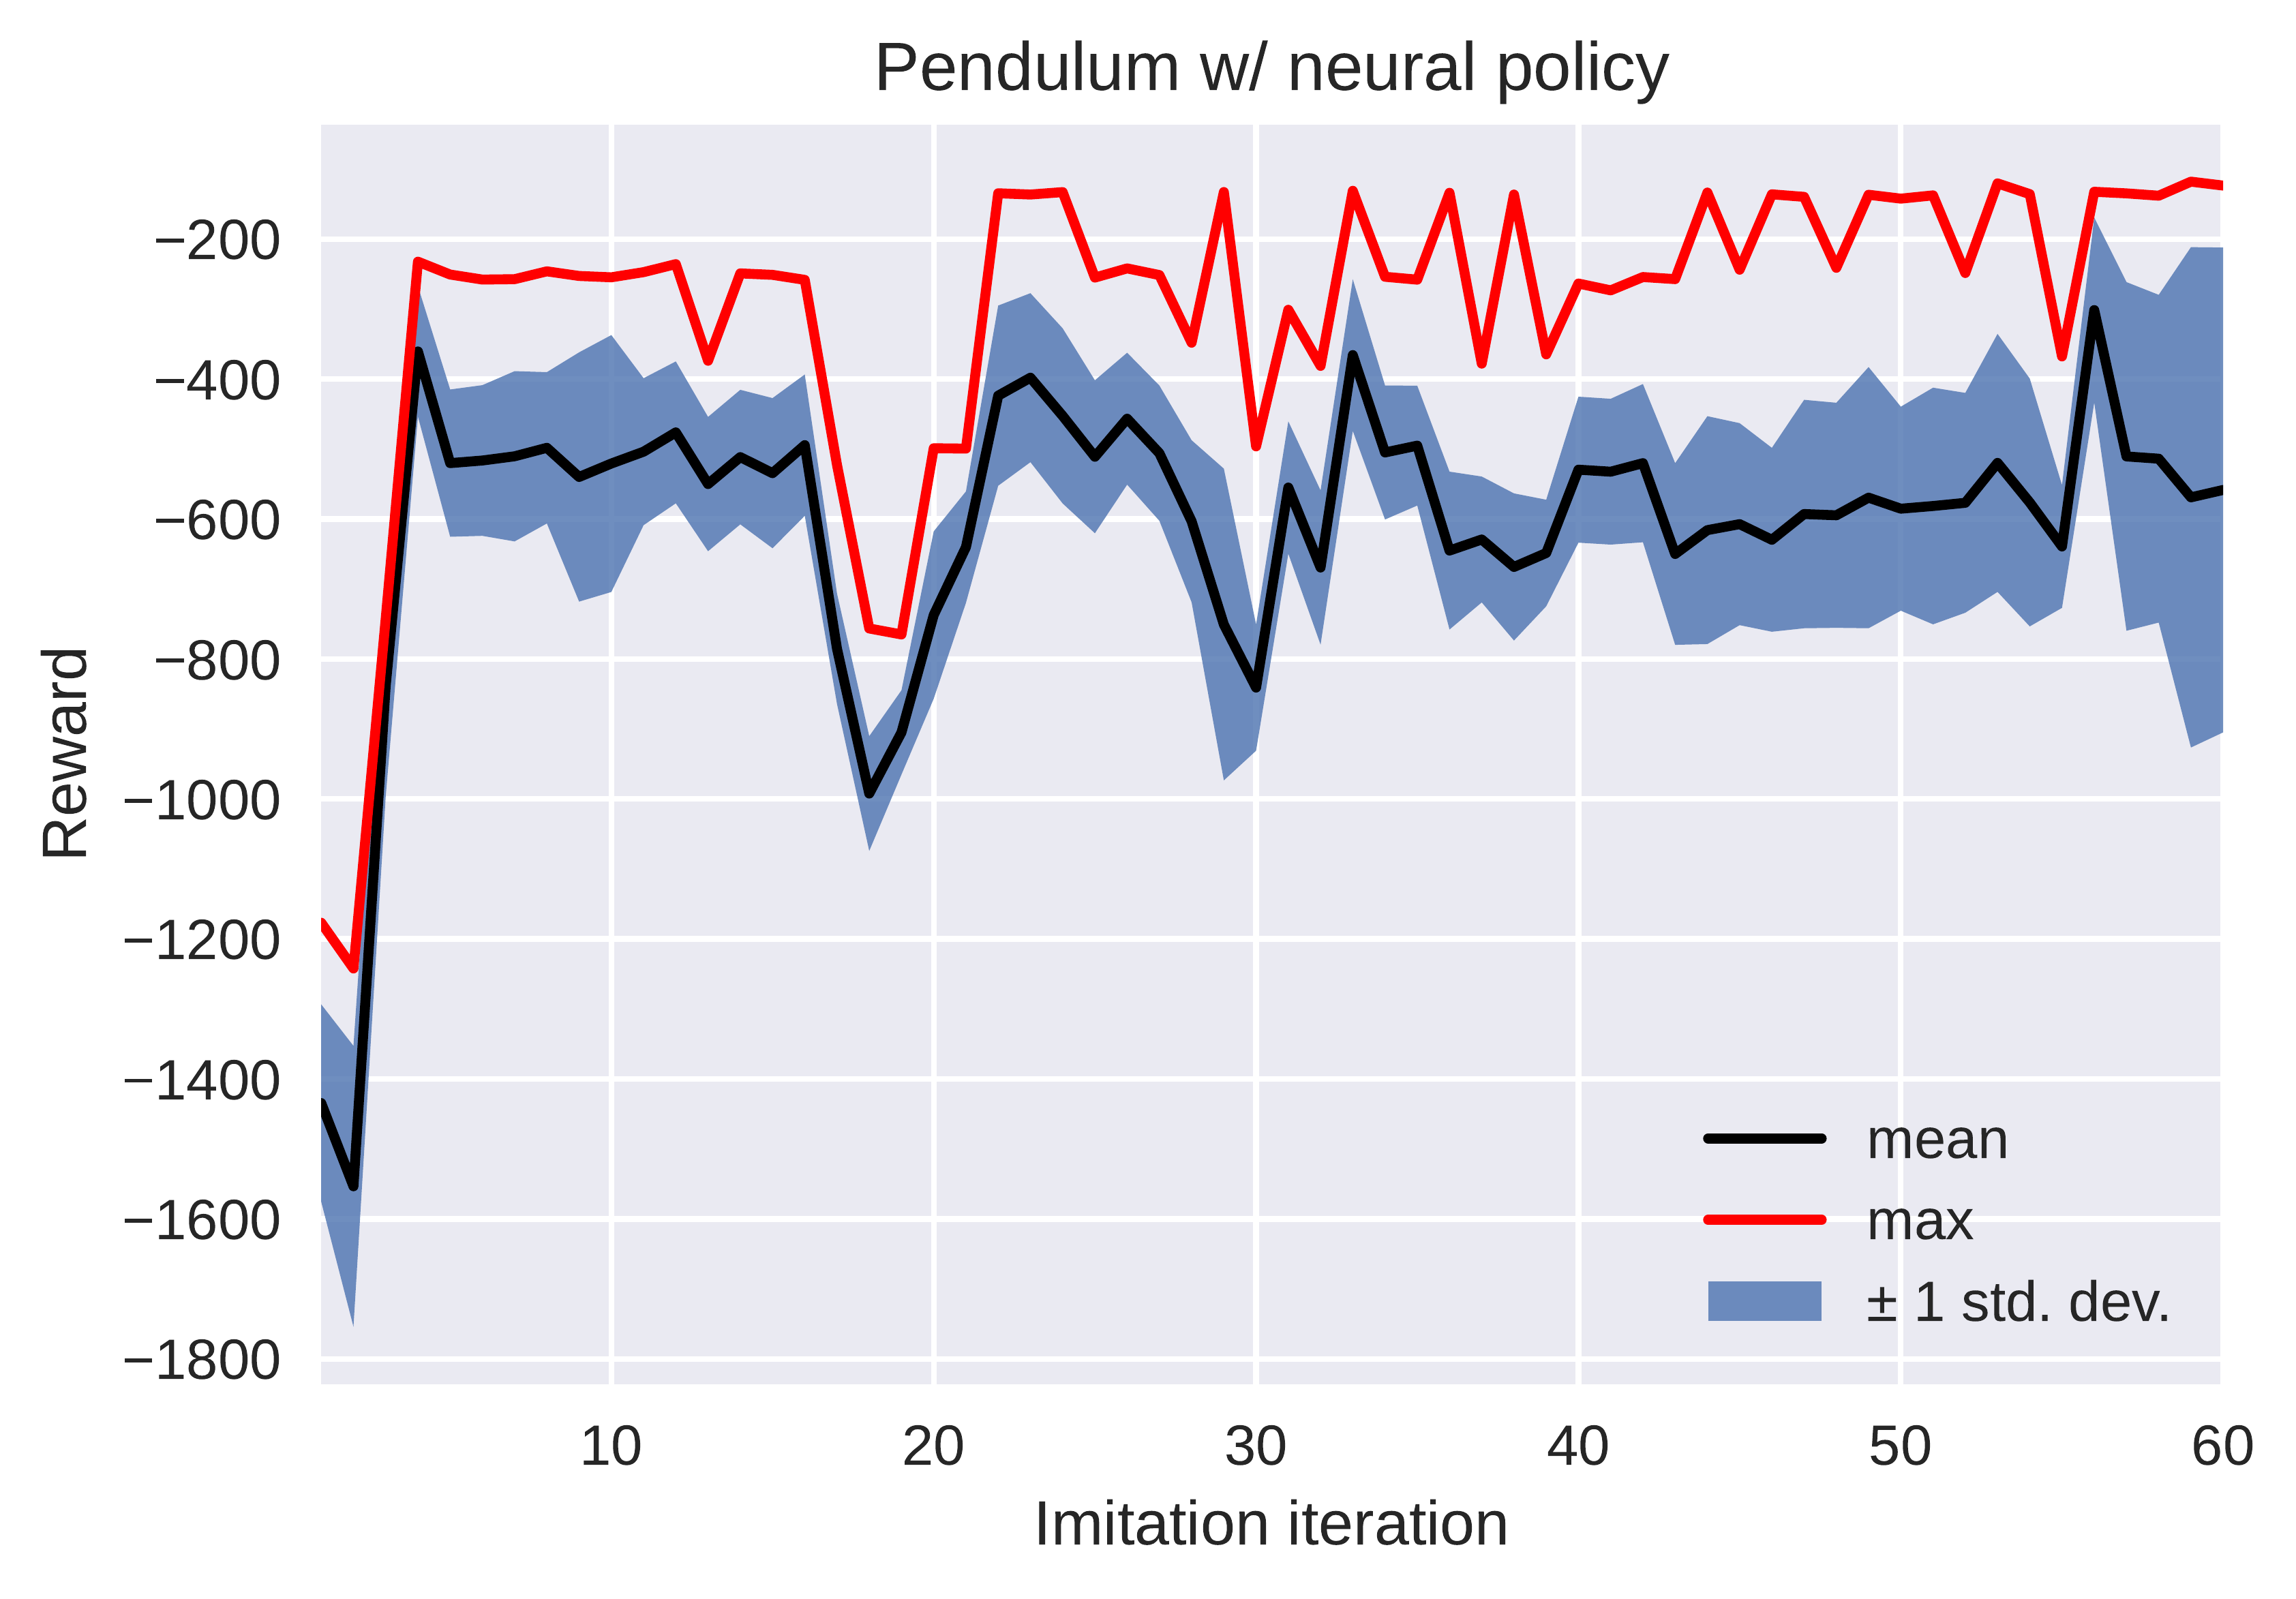
\includegraphics[width=0.37\textwidth]{images/performance.png}
      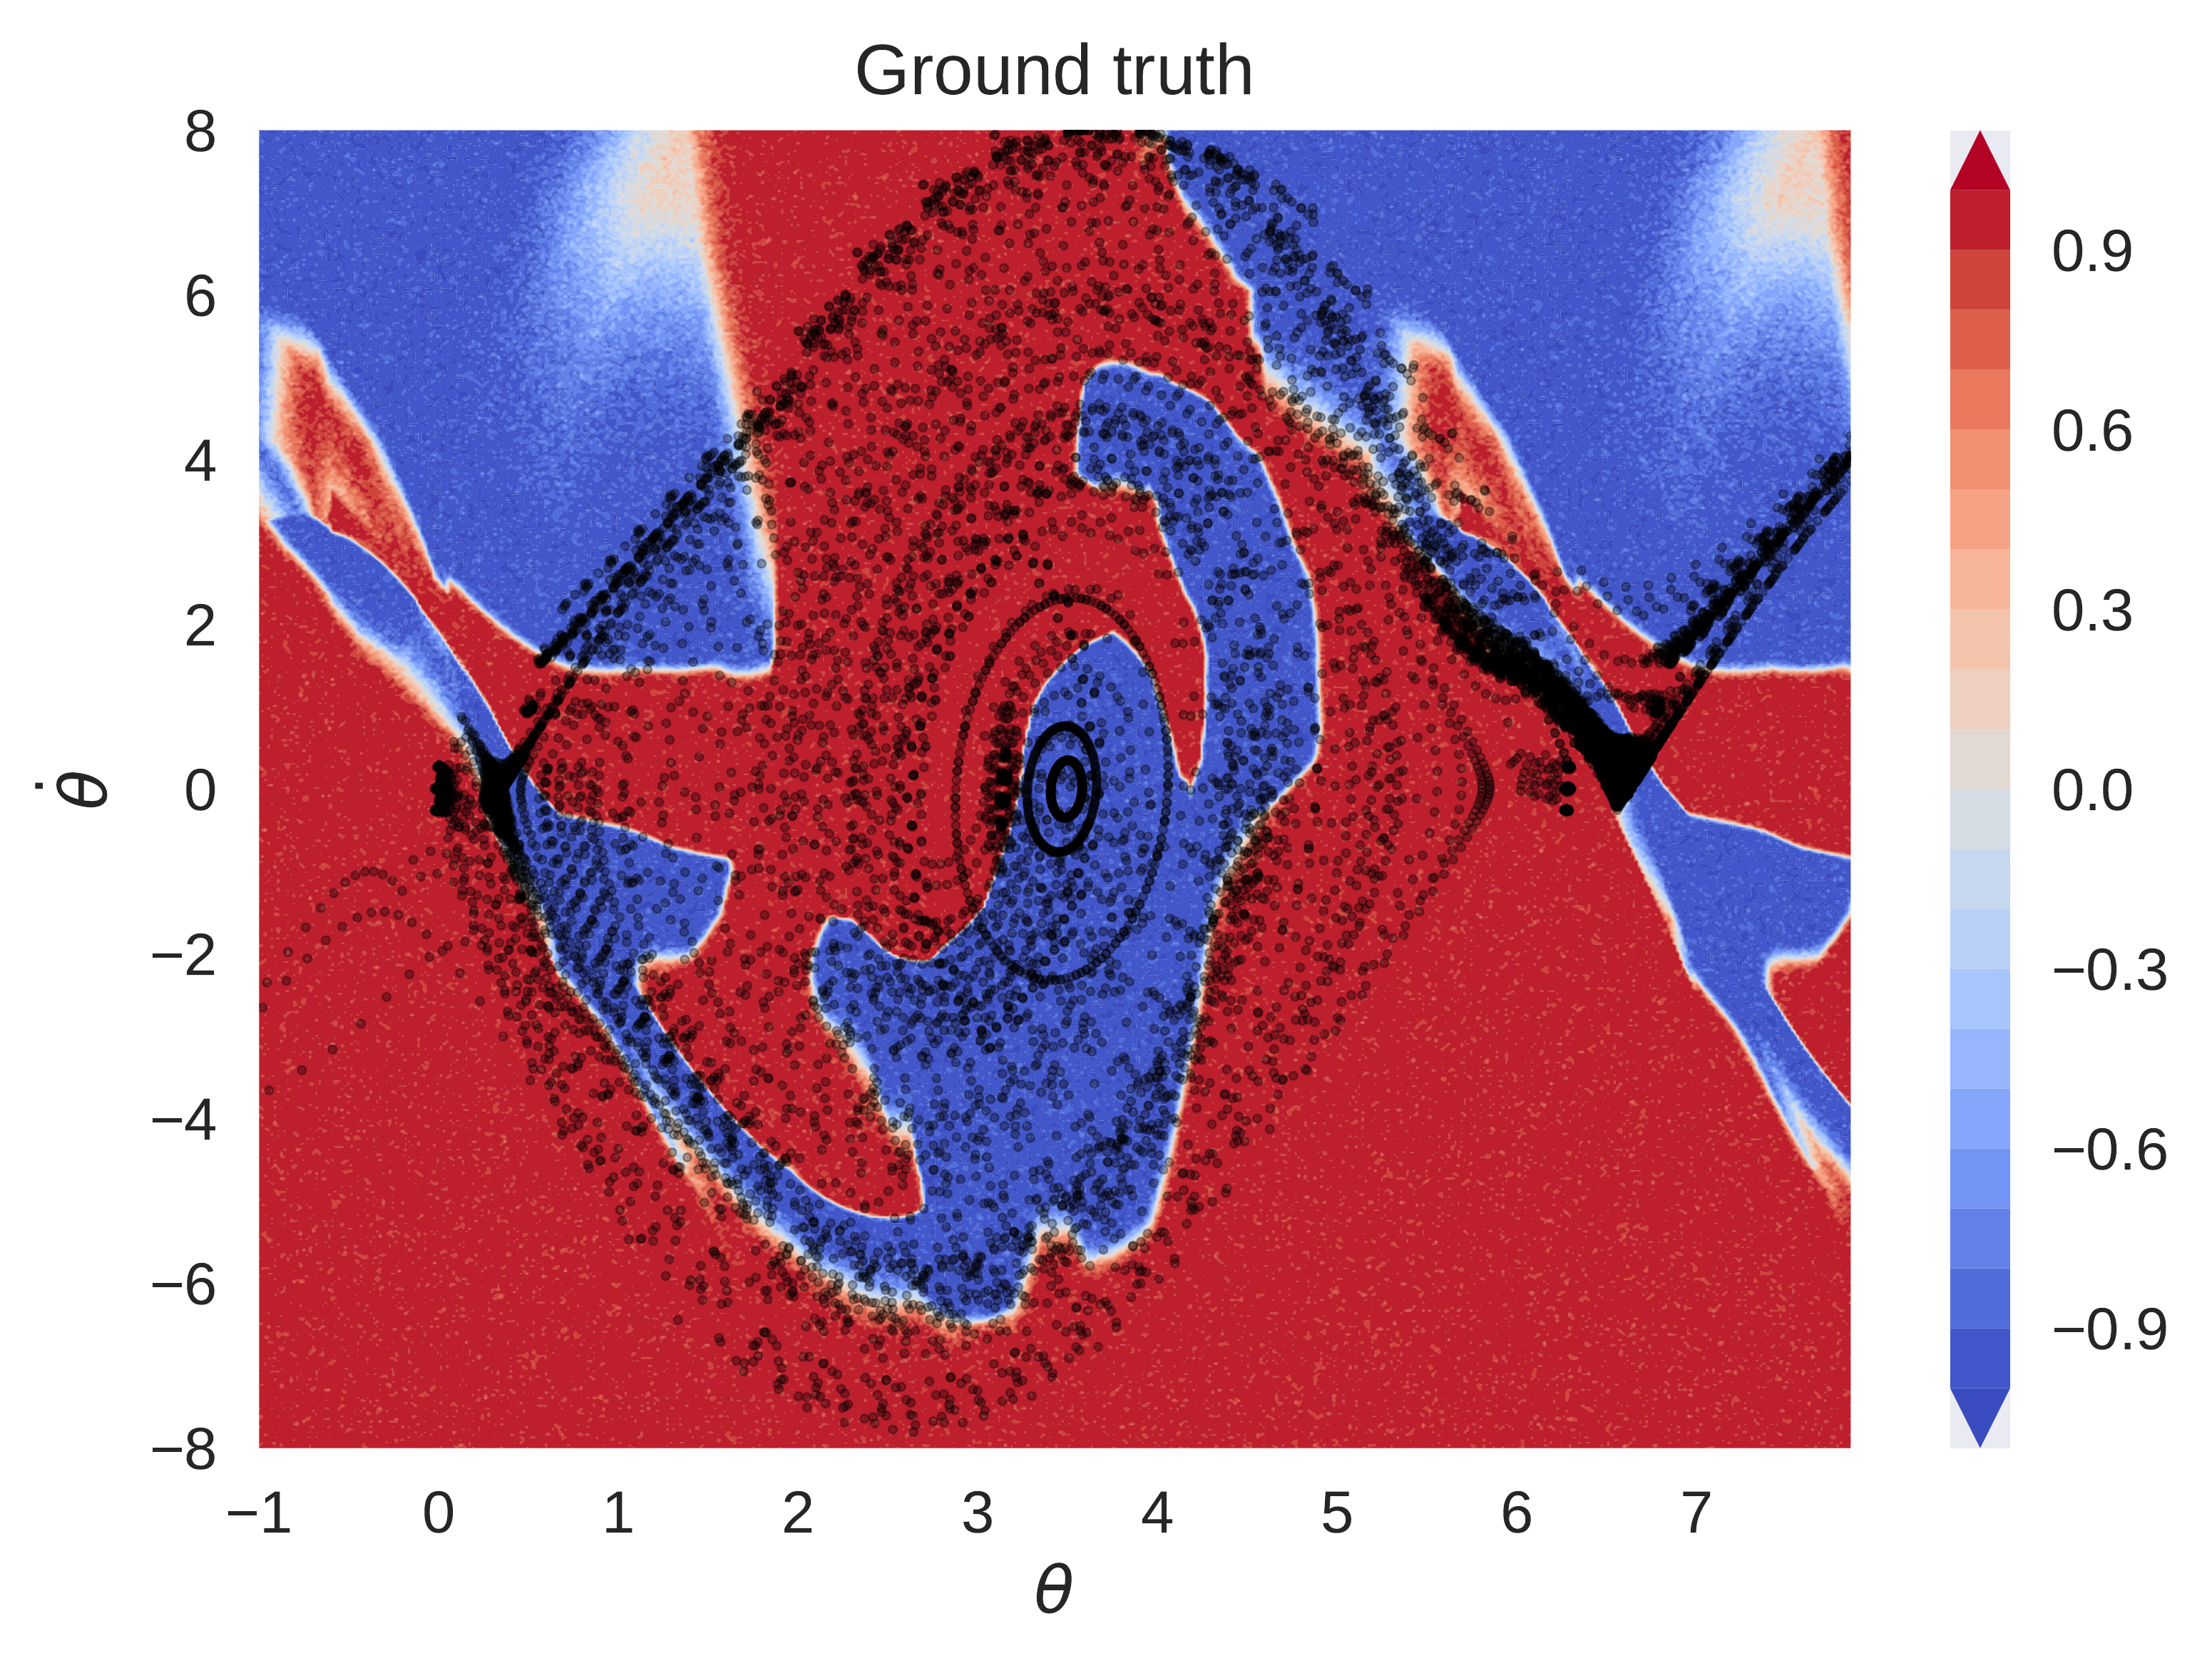
\includegraphics[width=0.37\textwidth]{images/groundtruth.png}
      
      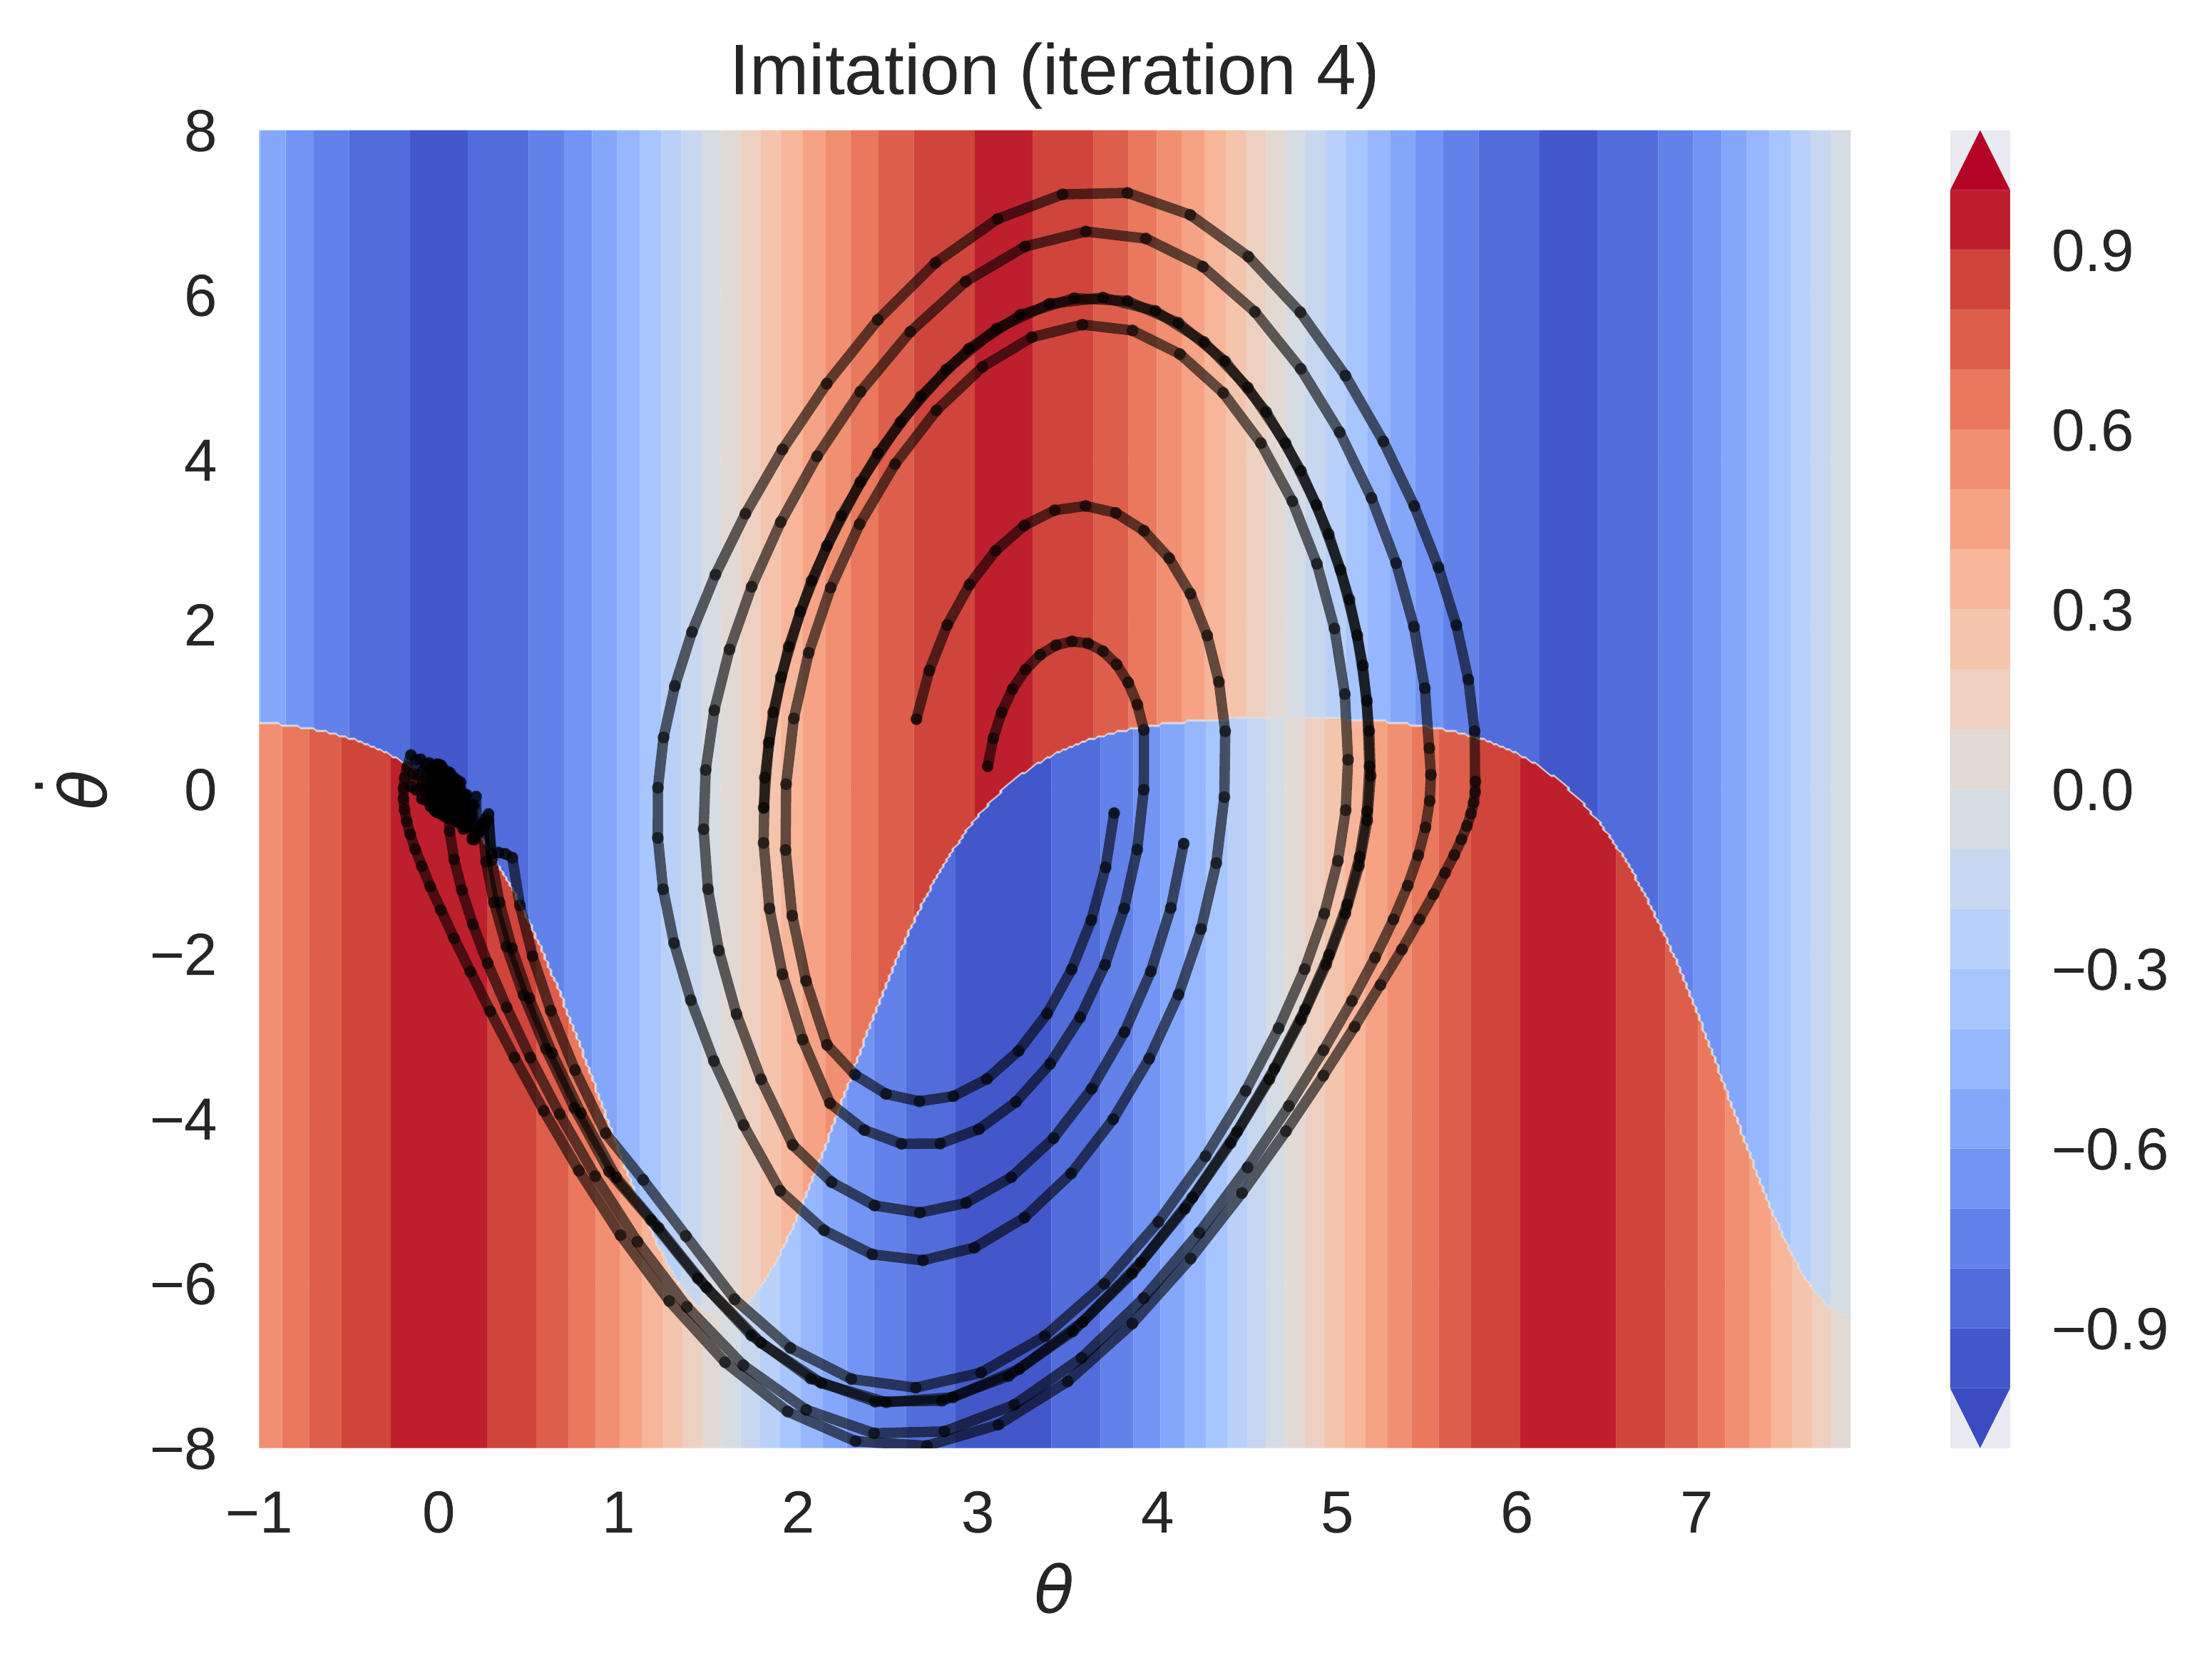
\includegraphics[width=0.37\textwidth]{images/imitation4.png}
      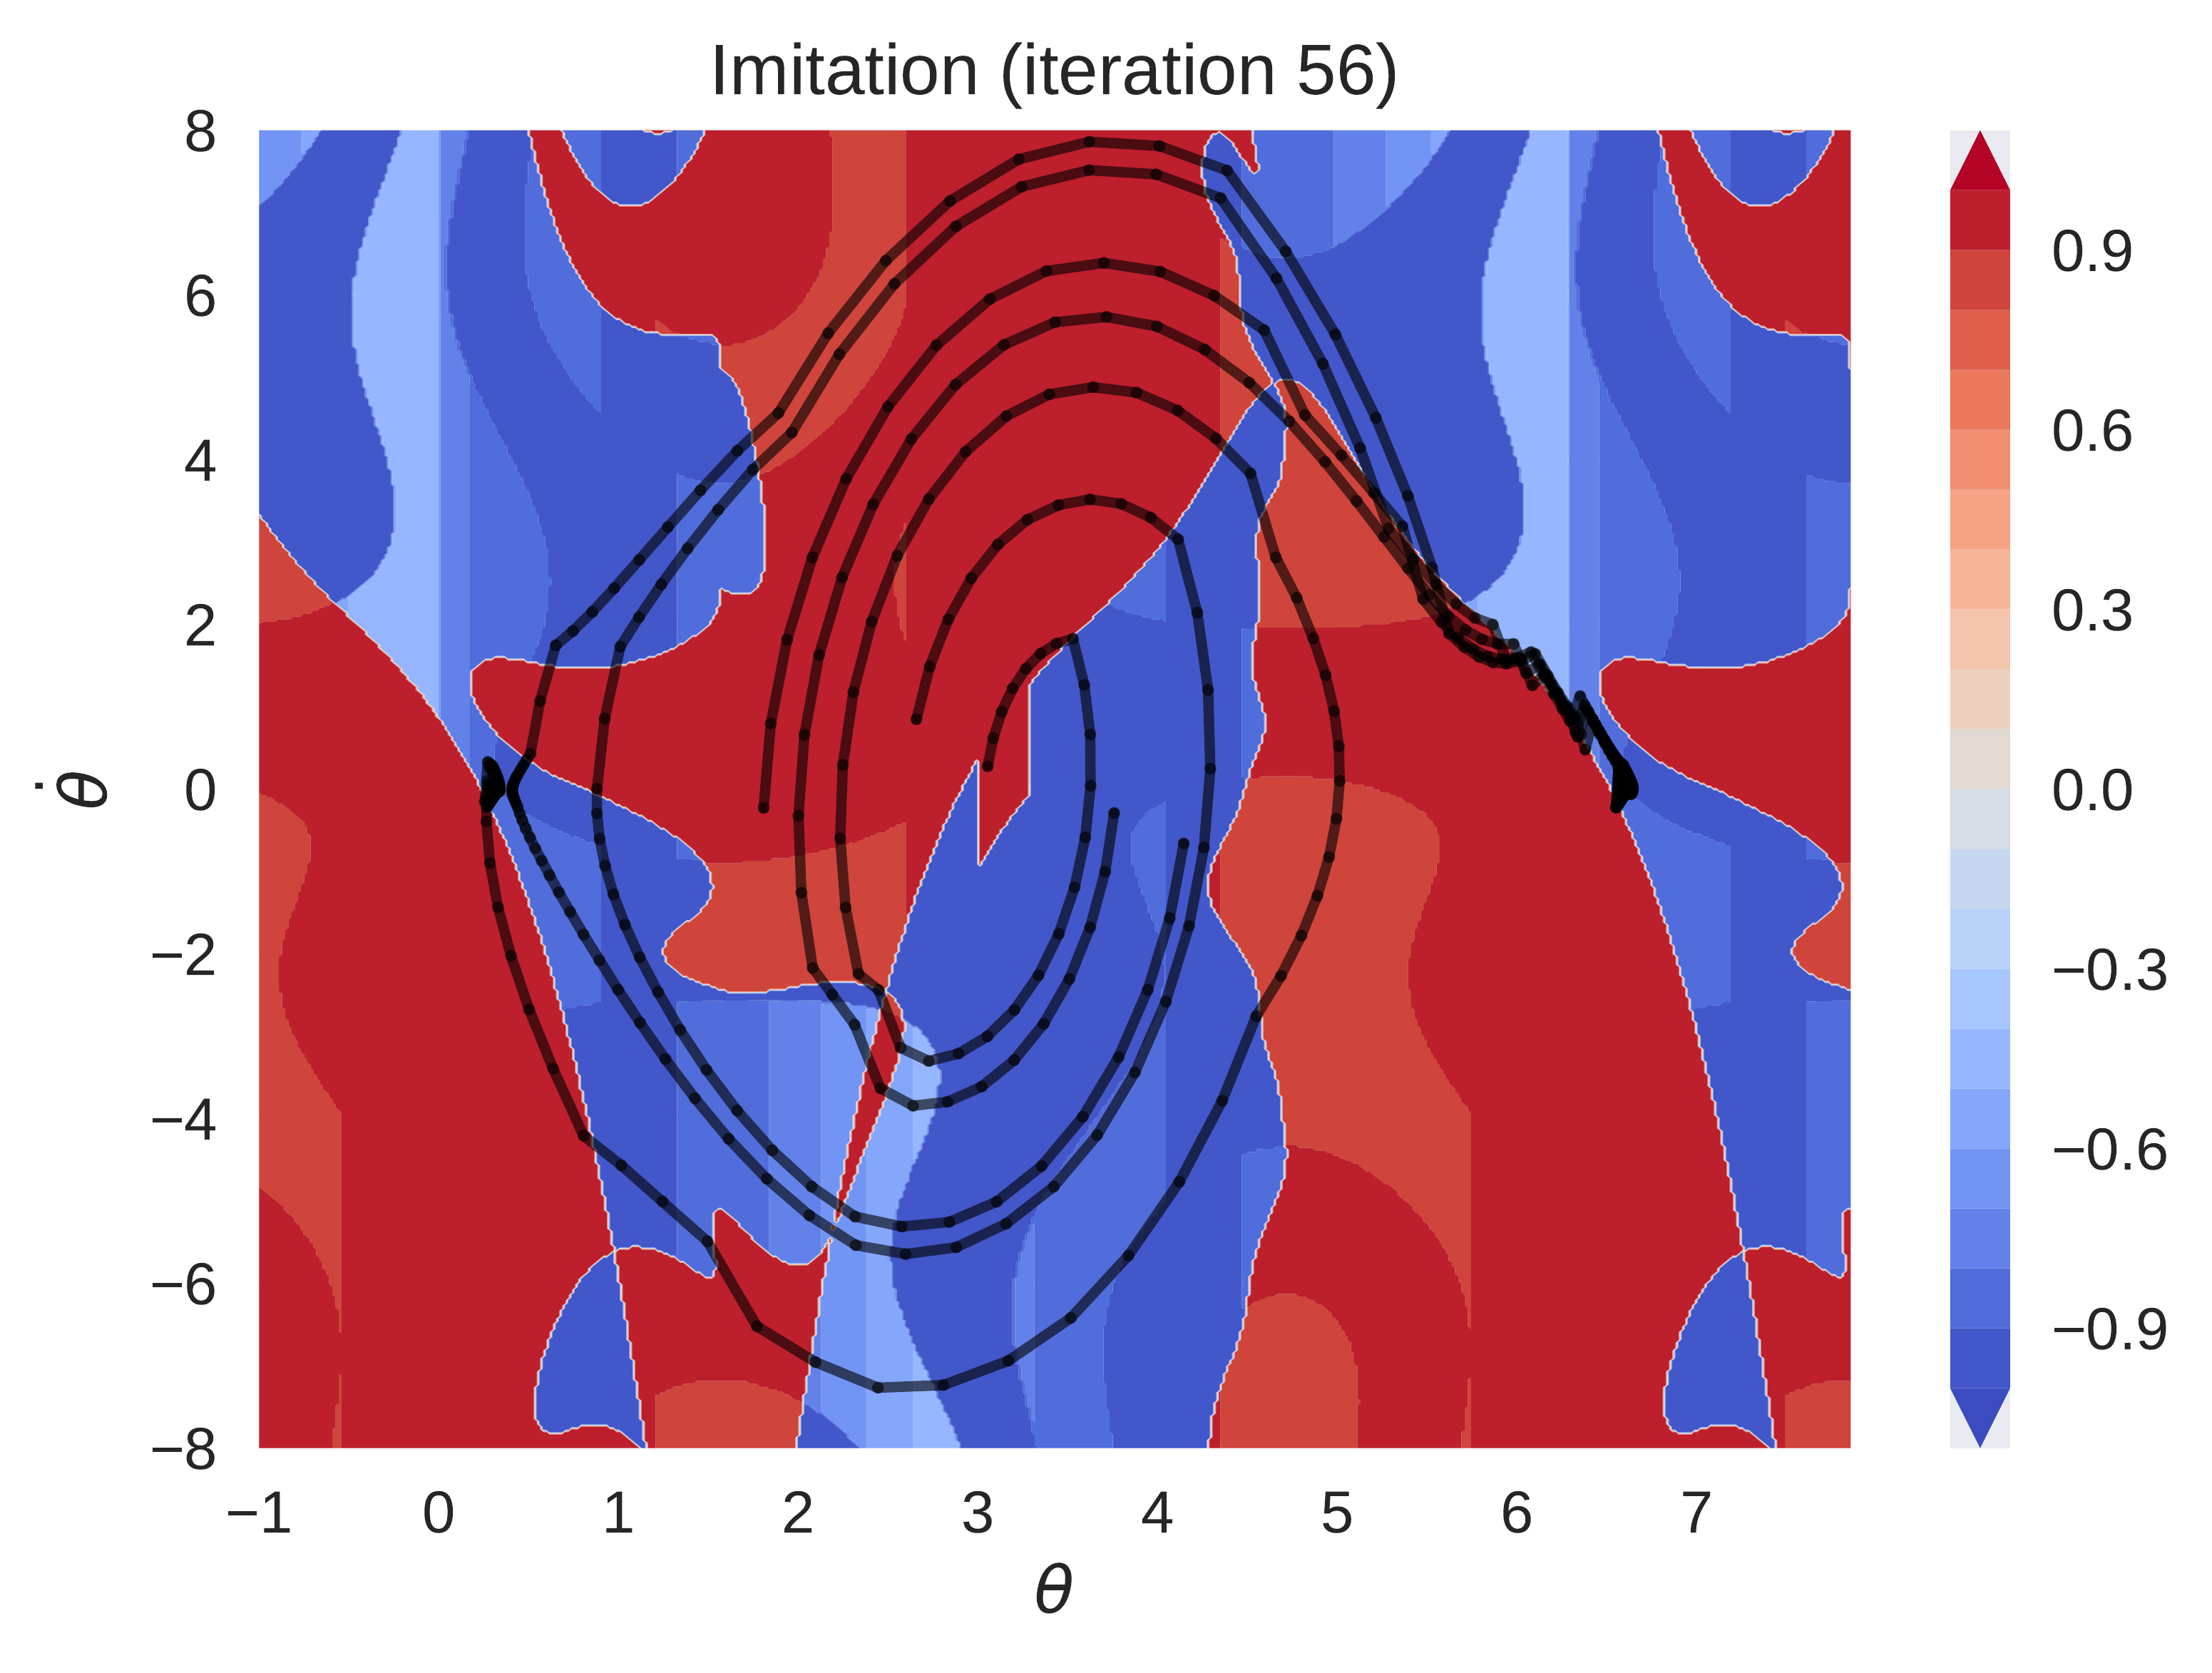
\includegraphics[width=0.37\textwidth]{images/imitation56.png}
    \end{figure}
    
\end{frame}

\begin{frame}{Summary}
    \begin{itemize}
        \item The Imitation-Projected Programmatic Reinforcement Learning framework integrates reinforcement learning with structured policy representations.
        \item We propose an extension to the framework, which we argue is key when scaling to more complicated structured spaces such as DSLs.
        \item Our experiments show that, despite using a simple local search heuristic which generates quite a few semantically identical candidates, interesting and/or complex solutions can be discovered across multiple iterations of interactive search.
    \end{itemize}
\end{frame}

\begin{frame}{Future work}
\begin{itemize}
    \item Integrate synthesis and learning steps, i.e. outer loop.
    \begin{itemize}
        \item How do we take advantage of discovered programs in the following reinforcement learning updates?
    \end{itemize}
    \item Examine policy decompositions and corresponding representations/DSLs.
    \begin{itemize}
        \item High-dimensional input processing.
        \item Decision making.
        \item Low-level control.
        \item Others?
    \end{itemize}
    \item Can certain reinforcement learning algorithms help discover structure better than others?
\end{itemize}
\end{frame}